%% Submissions for peer-review must enable line-numbering 
%% using the lineno option in the \documentclass command.
%%
%% Camera-ready submissions do not need line numbers, and
%% should have this option removed.
%%
%% Please note that the line numbering option requires
%% version 1.1 or newer of the wlpeerj.cls file, and
%% the corresponding author info requires v1.2
\documentclass[fleqn,10pt,lineno]{wlpeerj}

\title{Edge-Optimized Threat Detection with Florence V2 for Autonomous Surveillance in Resource-Constrained Environments}

\author[1]{Cynthia Konar}
\author[2]{Diya Das}
\author[3]{Sweety Singh}
\author[4]{Dr. Subitha D}
\affil[1,2]{B.Tech CSE, Vellore Institute of Technology, Chennai, India}
\affil[3]{B.Tech CSE with CPS, Vellore Institute of Technology, Chennai, India}
\affil[4]{Assistant Professor Senior Grade 2, Vellore Institute of Technology, Chennai, India}
\corrauthor[4]{Dr. Subitha D}{subitha.d@vit.ac.in}


\begin{abstract}
Traditional surveillance systems struggle to detect contemporary security threats including disguised individuals or hidden weapons and flying drones especially when operating in unstable or restricted resource conditions. The proposed research employs a portable edge-optimized threat detection system based on Florence v2 Vision-Language Transformer and customized for military-grade object detection. Raspberry Pi 5 hosts the system for localized execution while the ESP32-S2 DevKit supports wireless alert transmission through ESP-NOW protocol. The Florence v2 model is adapted using Parameter-Efficient Fine-Tuning (PEFT) with Low-Rank Adaptation (LoRA), enabling high-precision performance with reduced computational overhead. The data collection method involving web scraping produced 12,000 images that were supplemented by manual annotations and GAN-based synthetic image generation for training purposes. The model achieved 88.02\% overall accuracy that outperformed YOLOv8 and Faster R-CNN CNN models by reporting validation scores of 70.92 and test scores of 67.10 in Mean Average Precision (mAP@50). The detection accuracy for the two threat classes Drone and Hand-Gun exceeded 100\%. After the training process, the model was quantized and pruned to optimize the size for real-time edge hardware operations (16.6s/frame at 38.4\% RAM and 50.9\% CPU usage). The ESP32-S2 module functions as an integrated system to transport vital alerts over extensive distances using a network structure that does not require cloud administration. The system can accomplish autonomous real-time surveillance across military borders, urban airspaces, and critical civilian infrastructures. 
\end{abstract}

%\keywords{Keyword1, Keyword2, Keyword3}

\usepackage{algorithm}
\usepackage{algpseudocode}
\usepackage{amsmath}
\setlength\mathindent{1.5in}
\usepackage{graphicx}
\usepackage{float}
\usepackage{subcaption}
\usepackage{caption}
\usepackage[sorting=none, style=ieee]{biblatex} 
\bibliography{reference} 


\begin{document}

\flushbottom
\maketitle
\thispagestyle{empty}

%\keywords{Keyword1, Keyword2, Keyword3}
\noindent \textbf{Keywords:} Automated Defense System, Real-Time Surveillance, Threat Detection, Vision-Language Model, Florence v2, Vision Transformers, ViT, Edge Computing, ESP32 Communication, Raspberry Pi Camera Module, Low-Power Monitoring, Camouflage Detection, Weapon Identification, Secure Long-Range Alerts, Military and Civilian Applications, Cost-Effective Security, Autonomous Response System, Context-Aware Detection, On-Device Threat Analysis, Portable Defense Solution, Advanced Embedded Surveillance

\section*{Introduction}
Defense mechanisms must develop innovative technologies because security threats spread at unprecedented speed in the current era. Security threats spread through metropolitan regions while also affecting distant military bases which caused damage to human life and infrastructure alongside social disturbances. Stand-alone solutions as well as traditional cloud services together with investigative personnel no longer satisfy the requirements of contemporary security assurance. These detectors cannot track sophisticated threats like hidden adversaries and camouflaged weapons along with aerial threats because they operate too slowly to stop rapidly occurring damage \cite{1}.
Portable threat detection systems must be developed to address the present security needs by providing quick threat identification capabilities and operational environment awareness at reasonable prices. Modern security systems operate in an economic detection accuracy spectrum because military-grade equipment produces exact results that public agencies cannot access nor basic detection methods identify missiles or camouflage structures \cite{2}. The cloud-based centralized infrastructure results in delayed threat avoidance because it does not support real-time protection \cite{3}.
There are multiple attempts to solve these problems through deep learning combined with vision-based detection solutions. These difficulties persist in enhancing dataset diversity as well as decreasing computing complexity and ensuring real-time performance under limited resource conditions. Research evaluations employing CNN-based object detection strategies on security surveillance data have demonstrated ineffective processing of large-scale video data in real time thus lowering security performance \cite{4}. Most object identification approaches fail to adapt properly in complex situations particularly within adversarial environments where they combine contextual reasoning with generalized pattern detection methods \cite{5}. The exploration of ViT-based models showed potential for superior object detection capabilities yet experts have not thoroughly tested its deployment potentials for security system applications \cite{2}. 

Our project presents an intelligent defense system with advanced AI integrated into a small hardware setup. Rather than using heavy, cloud-based configurations, we run the Florence v2 Vision Transformer model natively on a Raspberry Pi 5 — a small but powerful device. The system accurately identifies 13 military-relevant object classes — including aircraft, drones, missiles, grenades, hand-guns, rifles, pistols, knives, camouflage, fire, smoke, military vehicles, and soldiers with high accuracy even in complex situations. To wirelessly send alerts, we employ the ESP32-S2 Dev-Kit, keeping communication quick and efficient, and making the system completely portable and deployable in remote or mission-critical deployments.
The following are this paper's main contributions:
\begin{itemize}
    \item Created a realistic and varied dataset by mixing web-scraped images with GAN-synthesized synthetic data to improve model learning.
    \item Utilized the Florence v2 Vision Transformer to detect 13 military-relevant object classes: Aircraft, Drone, Missile, Grenade, Hand-Gun, Pistol, Rifle, Knife, Camouflage, Fire, Smoke, Soldier, and Military Vehicle — to accurately detect objects even in dense or complicated scenes at high accuracy.
    \item Applied quantization and pruning to reduce the model size from 1 GB to under 400 MB, enabling it to be deployed on low-power edge devices such as the Raspberry Pi 5.
    \item Deployed the optimized Florence v2 model on a Raspberry Pi 5 for local, real-time detection. Utilized an ESP32 module to wirelessly transmit results to a remote desktop, enabling fast alerts without relying on cloud connectivity — ideal for field or mission-critical environments.
\end{itemize}

\section*{Background}

Artificial intelligence technology made a quick progression that revolutionized the way objects get detected while establishing object detection as an essential component of contemporary surveillance and defense. The review analyzes deep learning methods and transformer-driven visual architectures together with Raspberry Pi edge processing and security alerts controlled by ESP32 devices. The combination of these technological domains produces the fundamental structure required to develop real-time alert systems with intelligence features which work for civilian as well as military needs.
\vspace{1em}

\noindent
\textbf{Deep Learning Models for Object Detection}

\noindent
The development of object detection technology has focused on CNN-based and YOLO architectural approaches during recent times. Research work starting with \cite{6} and continuing with \cite{7} and ending with \cite{8} established deep learning as the successor to traditional image processing which led to superior satellite and aerial object detection capabilities. The new approaches minimized human annotation requirements while giving access to instant detection operations. The optimization of YOLO variants with various modules like ELU, SE, deformable convolutions and SAHI is described in \cite{9}, \cite{10}, \cite{11}, \cite{12}, \cite{13}, \cite{14}, \cite{15}, \cite{16}, \cite{17}, \cite{18}, \cite{19}, \cite{20}, \cite{21}, and \cite{22}. ResNet's scale variance solution combined with its occlusion detection and clutter background analysis and small-object detection enhancement capabilities ensured better practicality. Systems relying on anchor-free features and attention-aware and optimized loss methods achieved enhanced precision and correct detection which makes these systems suitable for military observation alongside border control functions and emergency response tasks. An article analysis by \cite{13} determined how precision and speed trade-offs changed between YOLO and ResNet and RCNN models to meet different operational requirements.
\vspace{1em}

\noindent
\textbf{Transformer-Based Vision Models}

\noindent
Object detection underwent a transformative change through transformers because they gained the ability to process both global context and long-range dependencies. Surveillance systems have benefited from Vision Transformers (ViTs) and hybrid CNN-transformer model approaches which were implemented in seven studies including \cite{5}, \cite{23}, \cite{24}, \cite{25}, \cite{26} and \cite{21}, \cite{17}. Raw video and unstructured SAR imagery can be processed effectively by these models which achieve high accuracy levels even when noise and shape deformations or blockages exist. Defense systems benefited from weapon identification and behavior tracking and camouflage detection capabilities which ViTs delivered alongside explainable and robust and ethical features. The detection accuracy of systems remained intact when self-supervised and few-shot learning methods were presented through \cite{24} and \cite{26} to the field. The integration of transformers with deformable convolutions along with attention modules in \cite{5} and \cite{19} brought extraordinary improvements to both real-time aerial detection and multi-object tracking at combat zones and autonomous drone operations.
\vspace{1em}

\noindent
\textbf{Edge Deployment Strategies Using Raspberry Pi}

\noindent
The deployment of detection systems on Raspberry Pi types of minimal hardware received examination in research conducted by \cite{3}, \cite{17}, \cite{28}, \cite{2}, and \cite{29}. Researchers presented the combination of MobileNet architecture with Mask R-CNN along with edge AI frameworks which perform local high-resolution input processing. The research provided continuous real-time performance through minimized delay and power usage requirements which made such systems deployable for field operations. \cite{2} showed how device-based processing protected privacy while cutting down transmission fees and \cite{3} and \cite{27} established basic principles for camera and sensor usage in mobile monitoring stations. The design configuration for edges established self-governing monitoring systems that operated more efficiently without requiring heavy dependence on backend resources which brought benefits for military operations in locations with minimal connectivity.
\vspace{1em}

\noindent
\textbf{Communication Frameworks Utilizing ESP32 for Secure Long-Range Alerts}

\noindent
The studies conducted by researchers about wireless communication illustrated security alongside power efficiency methods as per references \cite{30}, \cite{29}, and \cite{36}. ESP32 created an effective method to transmit peer-to-peer data securely between restricted systems while delivering real-time alerts. The combination of ESP-NOW protocol and Wi-Fi/Bluetooth transmission framework allowed signals to travel across large distances using energy-efficient and quick methods. As part of surveillance networks the system functioned to create autonomous networks that transmitted intelligence without human agents. Operational integrity requires decentralized communication according to \cite{29} and \cite{36} so self-operating threat detection systems become possible in national security applications.

\vspace{1em}

\noindent
\textbf{Review on Research Gaps}

\noindent
Several essential research gaps persist across Vision Transformers (ViT) and YOLO-based models and hybrid architectures regarding their application in real-time and cost-efficient portable Automated Defense Systems which would serve military as well as civilian purposes:

\begin{enumerate}
    \item Lack of Edge-Optimized Vision-Language Models: The recent advancements through Florence v2 and ViTs have successfully extracted semantic and spatial video relationships yet their extensive resource requirements make them unfit for embedded threat analysis on ESP32 and Raspberry Pi systems. Literature today does not include simplistic yet field-compatible Vision-Language models which can conduct real-time contextual threat identification and autonomous conclusions during actual operations.
    \item Limited Integration of Context-Aware Detection in Low-Power Environments: The majority of research efforts concentrate on detecting objects within controlled environments with abundant resources at their disposal. The development of accurate camouflage detection systems under various lighting conditions needs further work on low-power monitoring devices. Embedded platforms avoid dealing with scene semantics complexity because they have limited computational capabilities.
    \item Insufficient Focus on Portable and Scalable Defense Solutions: Remote and mobile deployments cannot utilize existing surveillance systems that depend on cloud connectivity or high-end GPUs. Research on edge computing-based surveillance systems which provide real-time alert notifications with security and speed preservation remains limited and scarce.
    \item Underdeveloped Explainability and Ethical Transparency in Real-Time Defense Systems:Multiple transformer-based defense applications operate as black boxes despite rising interest in XAI (Explainable AI). Issues about trust and accountability together with bias remain significant because of unknown system operations which affect weapon recognition and civilian monitoring. Additional study must take place to merge explainable visual outputs and transparent outputs with real-time systems before ethical deployment becomes possible.
    \item Delayed Reaction Time in Autonomous Response Systems: The ability to detect threats together with immediate defensive actions remains limited throughout almost all systems even though object tracking and action recognition have developed. The current systems experience delays because they need off-device processing or inefficient inference pipelines for execution.
\end{enumerate}

Addressing these research gaps presents an opportunity to design and implement a new automated defense system which integrates real-time Vision-Language models with edge computing and secure ESP32-S2 communication within affordable context-based surveillance operations. Such a system represents a fundamental transformation for treating threats in military and civilian applications where it delivers autonomous responses together with interpretation capabilities despite limited resources.




\section{Proposed Methodology}

This system implements a contemporary structure which detects threats in real-time with advanced neural learning methodologies together with artificial intelligence modeling and synthesized data generation and distributed processing technology. The system initiates an advanced dataset generation process that extracts frames from YouTube videos for the collection of high-quality images. Roboflow plays a role in manual labeling of images to create a training set suitable for supervised learning. The lack of specific class images due to military regulations can be addressed by implementing Generative Adversarial Networks to produce high-quality synthetic images before adding controlled illumination and viewpoint along with varied background complexity to increase training capabilities and detection precision. The additional data helps to enhance the model's generalization ability both within this application and standard real-world deployments.  

The proposed system utilizes Florence V2 Vision Transformer (ViT) model as its base since it demonstrates superior computer vision capabilities. A fine-tuning process takes place through the joint dataset containing real images along with images generated through GAN for enhancing threat detection abilities. The pre-trained Florence V2 model receives a reduction in computational expenses through Quantization and pruning techniques that maintain its accuracy performance. Data from the completed model is stored securely with Safe Tensors serialization while maintaining high efficiency during I/O operations and eliminating conversion requirements. A Raspberry Pi 5 board with high-definition camera module operates the deployment configuration to record live video streaming. The deployment takes place on the device itself for quick processing that requires low latency during critical operations. The quantization and pruning techniques enable efficient computation thus allowing system operation under this platform. Near real-time operation remains achievable with the limited resources of Raspberry Pi. A ESP32S2 dev communication module exists in the system to support remote monitoring along with alert transmission to control centers. A wireless operating method with minimal power requirements enables extended detection event transmissions which makes the system functional in remote locations with limited infrastructure support. Remote monitoring systems receive threat detection alerts from inference results which enables them to take appropriate actions at the proper time. The performance evaluation loop operates in real-time to measure precision and recall and F1-score and latency which help determine the efficiency and robustness of detection. Continuous GAN-based synthetic data generation and model optimization happens through deployment feedback learning for maintaining response to changing threat conditions in military environments. The system maintains ongoing functionality through its relentless development pattern that ensures its operation within scarce resource areas combined with changing conditions. 

\subsection{Overall System Architecture}

A reliable threat detection system is built through the project architecture which integrates three functional components from data collection to model training and edge deployment in Fig.~\ref{fig:overall-arch}. The project process begins with extracting threat-related video images through manual screenshots from YouTube videos that are followed by detailed label creation through the Roboflow platform for developing organization-based datasets. Through Generative Adversarial Networks (GANs) synthetic image generation the project addresses limited data availability in particular classes by expanding dataset diversity which allows the model to accurately predict in authentic applications. The V2 version of Florence operates using a Vision Transformer architecture to process a training dataset consisting of real images and synthetic images. The model receives optimization through the Safe Tensors format and quantization and pruning strategies to decrease processing requirements without compromising performance output. 

The optimized model executes in real time through a deployment on Raspberry Pi 5 along with its camera module functioning to process and detect threats in local video streams. The inference happens at the edge through this method which provides high speed results without internet connections enabling remote and critical applications. The Raspberry Pi triggers an alert by sending messages through an ESP32-S2 communication module which uses ESP-NOW protocol. ESP-NOW enables fleet communication between devices through a fast protocol that delivers efficient power usage and operates without infrastructure within reasonable distance ranges. Real-time threats alerts move from the system to a distant monitoring station which enables quick responses. The system becomes more efficient through performance tracking of precision, recall and inference time measurements and gets better through field deployment feedback that uses synthetic data expansion and model reparameterization for accuracy maintenance in changing military surroundings. 

\begin{figure}[H]
    \centering
    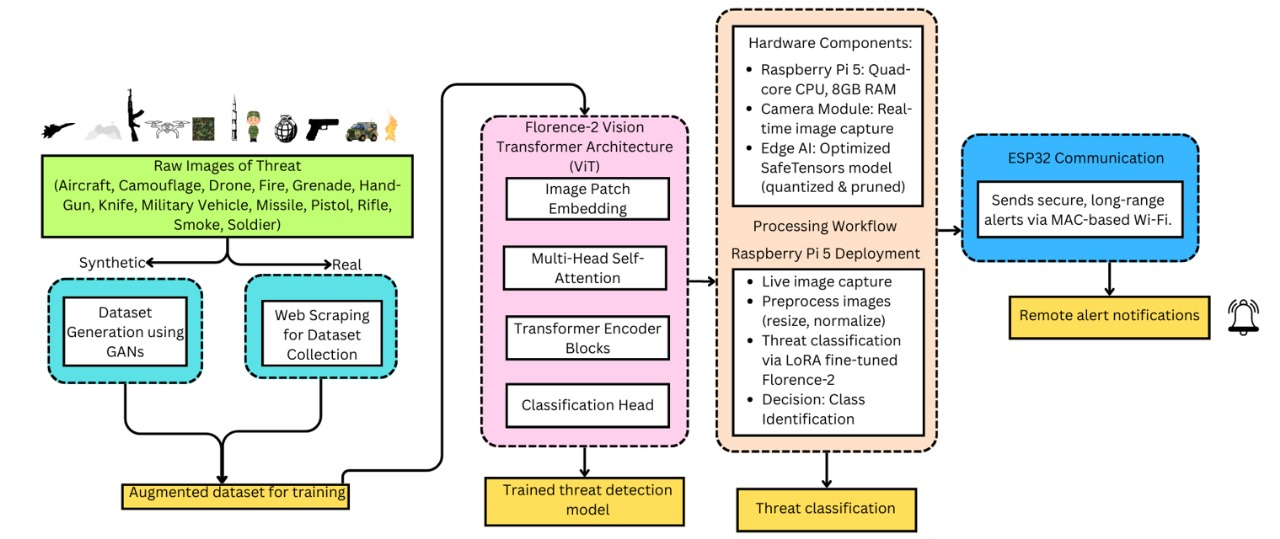
\includegraphics[width=1\linewidth]{overall_architecture.jpg}
    \caption{Overall Architecture of Transformer-Based Threat Detection System  }
    \label{fig:overall-arch}
\end{figure}

\subsection{Data Collection}

Data collection process is the core of our deep learning model in which the availa bility of a big and diverse dataset is critical to successful performance. In our project, we addressed the issue of scarce data availability by integrating the process of synthetic data generation using GANs and real data collection through web scraping. The dataset contains images of aircraft, missiles, guns, and other weapons, with labeling carried out through Roboflow for proper annotations. 

The application of GANs to synthetic data addresses cases where real images are hard to come by due to security, access, or ethical constraints. Merging web-scraped data into this exposes the model to a wide range of visual contexts, which aids in ro bustness and generalization.  

\subsubsection{GAN (Generative Adversarial Network) Image Generation}

A restricted number of images related to object scarcity were produced using Generative Adversarial Networks (GANs). The implemented method generated photographic computer simulations that represented military equipment such as firearms as well as aerial vehicles and explosive devices. During initial dataset development stages GANs functioned by filling classes that lacked sufficient accessible images or proved hard to obtain from public databases. Certain features of military scene synthesis using GANs proved challenging to recreate realistic results so this approach was intentionally restricted mainly to specific situations. Various experts reviewed the generated images to confirm realistic visual elements before final approval to include them in the dataset. Despite being used in a smaller capacity compared to other sources the modeling of GAN images successfully increased the diversity in the dataset and filled gaps within specific categories. 

GANs represent deep learning designs which create authentic synthetic data by learning the original distribution of real-world datasets. GANs as defined by Goodfellow et al. in 2014 involve two neural networks named G and D which play against each other in a zero-sum game format. The game notes synthetic data creation from the generator with simultaneous discrimination of real and synthetic data by the discriminator. Through their adversarial relationship the networks simultaneously enhance their capabilities until they generate high-quality synthetic output. The generator receives random noise z from the latent space before using it to create data sample G(z) such as images. The discriminator applies its analysis to check the generated output against training data samples to calculate a real or nonreal probability score. During operation the generator develops capabilities to generate data samples which imitate authentic samples.  

The optimization objective for the discriminator D and generator G can be defined as: 

\begin{equation}
\centering
\min_G \max_D V(D, G) = \mathbb{E}_{x \sim p_{\text{data}}(x)} \left[ \log D(x) \right] + \mathbb{E}_{z \sim p_z(z)} \left[ \log \left(1 - D(G(z)) \right) \right]
\end{equation}

Where:

\begin{itemize}
    \item $x$ is a real sample drawn from the data distribution $p_{\text{data}}(x)$.
    \item $z$ is a noise vector sampled from the prior distribution $p_z(z)$.
    \item $G(z)$ is a synthetic sample generated by the generator $G$ using the noise vector $z$.
    \item $D(x)$ is the probability score assigned by the discriminator $D$, indicating how "real" the sample $x$ is.
\end{itemize}

The training process is to iteratively update both the networks until the discriminator cannot tell real and fake samples apart, i.e., the generator has learned to map the data distribution well.

GAN architecture builds a system that produces high-resolution pictures through layerby-layer up scaling and image sharpening capabilities. The network design for both discriminator and generator consists of CNN layers suitable for processing images. The Generator network processes noise vectors by adding fully connected layers followed by transposed convolutional layers that expand the image dimensions in a detailed manner. Training stability is maintained through batch normalization while ReLU functions bring nonlinearities to the model. As a CNN device the Discriminator receives information from down sampled images while determining their authenticity traits. The convolutional layers develop hierarchical features by using more feature maps which are controlled through LeakyReLU to prevent dying neurons during training. During the final step of the operation the sigmoid activation establishes a probability to determine if the input image is genuine or not. 

\begin{algorithm}
\caption{Generator Network, Discriminator Network, and Training Process}
\label{alg:gan}
\noindent\textbf{Generator Network}
\begin{algorithmic}[1]

\State \textbf{Input:} Latent vector $z \in \mathbb{R}^{\text{latent\_dim}}$
\State Dense(1024) $\rightarrow$ ReLU
\State Dense($128 \times 8 \times 8$) $\rightarrow$ ReLU
\State Reshape to $(128,\ 8,\ 8)$

\For{$i = 1$ to $3$}
    \State ConvTranspose2D(filters $/ 2^i$, $4 \times 4$, stride=2, padding=1)
    \State \hspace{2em}$\rightarrow$ BatchNorm $\rightarrow$ ReLU
\EndFor

\State ConvTranspose2D(3,\ $4 \times 4$, stride=2, padding=1) $\rightarrow$ Tanh
\State \textbf{Output:} Generated image $\in \mathbb{R}^{3 \times 64 \times 64}$

\end{algorithmic}

\vspace{1em}
\noindent\textbf{Discriminator Network}
\begin{algorithmic}[1]

\State \textbf{Input:} Image $\in \mathbb{R}^{3 \times 64 \times 64}$

\For{$i = 1$ to $3$}
    \State Conv2D(filters $\times 2^i$, $4 \times 4$, stride=2, padding=1)
    \State \hspace{2em}$\rightarrow$ BatchNorm $\rightarrow$ LeakyReLU(0.2)
\EndFor

\State Dense(1) $\rightarrow$ Sigmoid
\State \textbf{Output:} Probability $\in [0,\ 1]$

\end{algorithmic}

\vspace{1em}
\noindent\textbf{Training Process}
\begin{algorithmic}[1]

\State Initialize Adam optimizers with $lr = 0.0002$, $\beta_1 = 0.5$, $\beta_2 = 0.999$

\For{each epoch}
    \For{each batch in training data}
        \State Train Discriminator on real and fake samples
        \State Train Generator to fool the Discriminator
        \State Log training progress and save checkpoints
    \EndFor
\EndFor

\end{algorithmic}
\end{algorithm}


This detailed pseudocode outlines the sequential processing of data through various layers, emphasizing the role of each component in the GAN architecture. 

Algorithm~\ref{alg:gan} presents the method used to develop and train GANs. The Generator receives latent vectors which it transforms into 64×64 RGB images through successive operations of dense and transposed convolution. The Discriminator analyzes images through LeakyReLU-activated convolutional layers that eventually classify input
images as either real or fake. The adversarial training linking the Adam optimizer allows the Generator to develop authentic images while requiring the Discriminator to detect these images. Training involves periodic checkpointing to track progress in addition to using batch-wise updates. 

\begin{algorithm}
\caption{Training Procedure for Generative Adversarial Network (GAN)}
\label{alg:gan_training}
\noindent\textbf{Input:} Generator $G$, Discriminator $D$, learning rate $\alpha$, batch size $B$, number of epochs $E$
\begin{algorithmic}[1]

\State \textbf{// Initialize model weights}
\State Randomly initialize weights of $G$ and $D$

\For{epoch $e = 1$ to $E$}
    \For{each batch $b$ in training data}

        \State \textbf{// Train Discriminator}
        \State Sample real data $x$ from dataset
        \State Sample noise vector $z \sim \mathcal{N}(0,\ 1)$
        \State $x_{\text{fake}} \gets G(z)$
        \State $D_{\text{real}} \gets D(x)$ \\textbf{Real data score}
        \State $D_{\text{fake}} \gets D(x_{\text{fake}})$ \\textbf{Fake data score}
        \State $L_D \gets - \left( \log D_{\text{real}} + \log(1 - D_{\text{fake}}) \right)$
        \State Update $D$ to minimize $L_D$

        \State \textbf{// Train Generator}
        \State Sample noise vector $z \sim \mathcal{N}(0,\ 1)$
        \State $x_{\text{fake}} \gets G(z)$
        \State $D_{\text{fake}} \gets D(x_{\text{fake}})$
        \State $L_G \gets - \log D_{\text{fake}}$
        \State Update $G$ to minimize $L_G$

        \State \textbf{// Log progress every 10 epochs}
        \If{$e \bmod 10 = 0$}
            \State Save model checkpoint
            \State Evaluate generated samples
        \EndIf

    \EndFor
\EndFor

\end{algorithmic}
\noindent\textbf{Output:} Trained Generator $G$ and Discriminator $D$
\end{algorithm}

Synthetic and web-based data acquisition methods give computer vision problems a solid solution to deal with data scarcity issues. GANs functions as a fundamental tool to develop high-quality diverse images for enhancing dataset diversity. The performance stability and improvement process utilize transposed convolutional layers
along with batch normalization methods. Web-scrapped real-world images serve multiple purposes by improving model generalization capabilities for real-world deployments. An end-to-end data acquisition system can be developed for highperformance machine learning models through this two-stage process.


This iterative process continues until the generator produces realistic images that the discriminator struggles to differentiate from real samples. The training scheme of Generative Adversarial Networks (GANs) comprises two neural networks according to Algorithm~\ref{alg:gan_training} where Generator G generates natural-looking outputs and Discriminator D, learns to recognize generated from authentic examples. The training cycle for each
weight update utilized genuine examples with synthetic outputs made by the Generator which the Discriminator detects to facilitate metric-based adjustments. The Generator undertakes an update process to acquire better capabilities in deceiving the Discriminator. Throughout each epoch the competing loop system executes through sessions of evaluation which measure progress.

\subsubsection{Web-Scraping}
Web scraping served as the main image acquisition method for the Military Base Object Detection dataset while collecting most of its images. The automated process of extracting images operated through public domain internet resources such as defense news outlets and open-source military archives and video repositories and public domain image libraries. Web scraping involved intelligent scripts that developed a system that selected and organized relevant images belonging to aircraft, missiles, military vehicles, handguns, rifles, drones, smoke, fire and other military objects. The selection process focused on acquiring pictures covering different background settings with diverse lighting effects and multiple camera views and object hiding situations. A large range of data types proved essential for developing an object detection model that exhibited strong performance in authentic operational settings. The images underwent labeling with precise bounding boxes through the Roboflow platform after completion of collection. The annotation team applied a standard approach to the entire dataset so the final annotations would be both precise and of high quality for training purposes. The midsection of our data collection plan consisted of web scraping because this methodology provided the extensive dataset necessary to create efficient models.

\subsection{Vision Transformer - Florence V2 Model}

The progress of deep learning methods made computer vision shift from convolutional neural networks (CNNs) to transformer-based models. Vision Transformers (ViTs) implement the self-attention approach from natural language processing for extracting extended image relationships. Photo recognition and detection functions along with segmentation capabilities benefit from this systematic worldwide visual understanding ability.

The Microsoft Azure AI-developed Florence-2 system Fig.~\ref{fig:florence-arch} equips Vision Transformers with multi-modal operations to deliver superior results for vision-language applications including captioning and object detection and border identification and image partition. The compact design of Florence-2 enables performance at levels or higher than Kosmos-2 while maintaining an efficient processing of image-text relations. The first ViT layers operate through embedding and patching to establish global awareness while both approaches differ in how they construct receptive fields.

\subsubsection{Theoretical Background}
\textbf{Patch Embedding:} The input image $X \in \mathbb{R}^{H \times W \times C}$ is divided into $N$ patches of size $P \times P$ with channels $C$:

\begin{equation}
N = \frac{H \times W}{P^2}
\end{equation}


Each patch is flattened and projected to a latent dimension $D$:

\begin{equation}
z_i = W_e \cdot x_i + b_e
\end{equation}

where $W_e$ is the learnable weight matrix, $x_i$ is the $i^\text{th}$ attend patch, and $b_e$ is the bias term.

\textbf{Positional Encoding:} To retain spatial information, positional embeddings $E_{pos}$ are added:

\begin{equation}
z_i = z_i + E_{pos}
\end{equation}

\textbf{Multi-Head Self-Attention (MHSA):} The self-attention mechanism computes attention weights by projecting tokens into query ($Q$), key ($K$), and value ($V$) spaces:

\begin{equation}
Q = z_i W_Q,\quad K = z_i W_K,\quad V = z_i W_V
\end{equation}


The attention output is given by:

\begin{equation}
\text{Attention}(Q, K, V) = \text{softmax}\left(\frac{Q K^T}{\sqrt{d_k}}\right) V
\end{equation}


\textbf{Transformer Block:} The standard block includes MHSA followed by a feed-forward network (FFN), each with residual connections and layer normalization:

\begin{equation}
\hat{z}_i = \text{LayerNorm}(z_i + \text{MHSA}(z_i))
\end{equation}

\begin{equation}
z_i = \text{LayerNorm}(\hat{z}_i + \text{FFN}(\hat{z}_i))
\end{equation}


\begin{algorithm}
\caption{Vision Transformer (ViT) Inference}
\label{alg:vit_inference}
\noindent\textbf{Input:} Image $I$ of size $(H, W, C)$, patch size $P$, number of transformer layers $L$
\begin{algorithmic}[1]

\State \textbf{// Divide image into patches}
\State $N \gets \frac{H \times W}{P \times P}$

\For{$i = 1$ to $N$}
    \State $Patch_i \gets \text{ExtractPatch}(I,\ i)$
    \State $Token_i \gets \text{Flatten}(Patch_i)$
\EndFor

\State \textbf{// Linear projection of patches}
\For{$i = 1$ to $N$}
    \State $Token_i \gets \text{LinearProjection}(Token_i)$
\EndFor

\State \textbf{// Add positional embeddings}
\State $Tokens \gets \text{AddPositionalEmbedding}(Token_1, \dots, Token_N)$

\State \textbf{// Pass through Transformer layers}
\For{$layer = 1$ to $L$}
    \State \textbf{// Multi-Head Self-Attention}
    \State $(Q, K, V) \gets \text{ProjectToQKV}(Tokens)$
    \State $Attention \gets \text{Softmax}\left( \frac{Q \cdot K^T}{\sqrt{d_k}} \right) \cdot V$
    \State $Tokens \gets \text{LayerNorm}(Tokens + Attention)$

    \State \textbf{// Feed-Forward Network}
    \State $FFN\_Output \gets \text{GELU}(Tokens \cdot W_1 + b_1) \cdot W_2 + b_2$
    \State $Tokens \gets \text{LayerNorm}(Tokens + FFN\_Output)$
\EndFor

\State \textbf{// Generate final prediction}
\State $Prediction \gets \text{OutputLayer}(Tokens)$

\end{algorithmic}
\noindent\textbf{Output:} Prediction $Prediction$
\end{algorithm}


Algorithm~\ref{alg:vit_inference} describes the operational sequence of Vision Transformer (ViT). The input image divides into fixed-size patches through segmentation and turns into single element tokens because of flattening. Linear projections reduce the tokens before positional embeddings are added to the result. The Transformer consists of multiple layers that combine the token sequence with multi-head self-attention and feed-forward network through normalization and residual connections. Finished output results appear from the output layer after processing all received tokens.

\begin{algorithm}
\caption{Multi-Modal Vision-Language Processing}
\label{alg:multimodal_vlp}
\noindent\textbf{Input:} Image $I$, Task Prompt $T$
\begin{algorithmic}[1]

\State \textbf{// Step 1: Encode Image using DaViT}
\State $ImageTokens \gets \text{VisionTransformer}(I)$

\State \textbf{// Step 2: Encode Text using BERT}
\State $TextTokens \gets \text{BERT}(T)$

\State \textbf{// Step 3: Concatenate Image and Text Tokens}
\State $InputTokens \gets \text{Concatenate}(ImageTokens,\ TextTokens)$

\State \textbf{// Step 4: Pass through Multi-Modal Encoder-Decoder}
\For{$layer = 1$ to $L$}
    \State \textbf{// Multi-Head Self-Attention on Input Tokens}
    \State $Q, K, V \gets \text{LinearProjections}(InputTokens)$
    \State $Attention \gets \text{Softmax}\left( \frac{Q \cdot K^T}{\sqrt{d_k}} \right) \cdot V$
    
    \State \textbf{// Feed-Forward Network}
    \State $FFN\_Output \gets \text{GELU}(Attention \cdot W_1 + b_1) \cdot W_2 + b_2$
    \State $InputTokens \gets \text{LayerNorm}(InputTokens + FFN\_Output)$
\EndFor

\State \textbf{// Step 5: Generate Textual Output}
\State $Response \gets \text{Decode}(InputTokens)$

\end{algorithmic}
\noindent\textbf{Output:} Textual Response $Response$
\end{algorithm}


Algorithm~\ref{alg:multimodal_vlp} describes the Florence-2 model’s unified vision-language inference process. The system deploys both DaViT-based Vision Transformer encoding for image processing to combine with BERT encoder processing of the task prompt. Image and text tokens join together into a single sequence that progresses through multiple layers with self-attention while using feed-forward processing methods. The model fuses both vision and language elements to conduct joint reasoning that leads to generating relevant text as its output. 

The Florence v2 model serves as visual architecture within the image that functions through transformer-based encoding for performing high-performance detection tasks. The model uses attention mechanisms together with hierarchical features to simultaneously perform classification and localization tasks that require dense prediction. The architecture contains three distinct elements for multi-scale patch extraction coupled with visual encoding to finish with an object detection head.

To begin with, the model receives image input which is divided into multi-scale patches that provide detailed visual information at different magnifications. The detection system achieves sensitivity toward image elements both at the local level and at the contextual level of the image through this method. The normalization process via Sigmoid function applies to these patches to both improve their learned features and prepare them for processing in the main network structure. The visual encoder 
represents the foundation of the architecture by utilizing a transformer block stack design. The visual encoder starts each block with LayerNorm as its initial process to achieve training stability through feature dimension normalization. A Multi-head SelfAttention (MSA) mechanism operates next in the process to provide the model with the capability to detect extended dependencies and contextual patterns across different image areas. Prior to another LayerNorm operation the self-attention process completes its execution.

\begin{figure}[H]
    \centering
    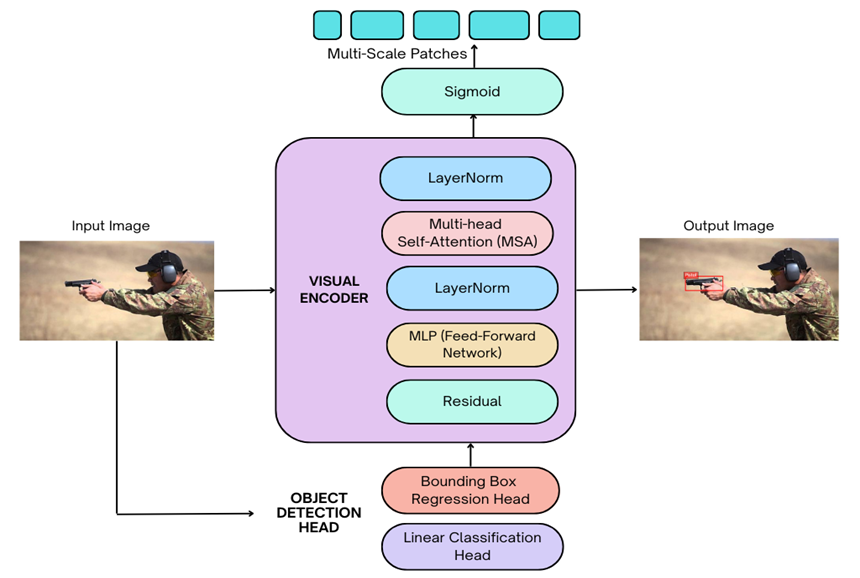
\includegraphics[width=0.75\linewidth]{florence_architecture.png}
    \caption{Model Architecture of Florence v2}
    \label{fig:florence-arch}
\end{figure}

A subsequent MLP (Feed-Forward Network) operation follows feature data to increase its non-linear capacity. The model's expressive power becomes stronger because this MLP contains linear transformations operated with activation functions alongside it. 
The transformer blocks include residual connections that support efficient gradient flow throughout backpropagation while making deep architectural designs feasible without gradient disappearance. Two functions exist for visual encoder output. The forward progress of the system produces an amplified output image representation that downstream functions including image captioning and retrieval can use. The object detection head accepts the output from the visual encoder which splits into two vital sections: a Bounding Box Regression Head and a Linear Classification Head alike. The bounding box regression head performs the task of identifying exact object positions in 
images through their spatial coordinates. The classification head gives each detected region object class probabilities to guarantee proper identification between localized entities. 

The architectural framework showcases transformer-based computer vision strengths through combined use of attention mechanisms and hierarchical patch embeddings and feed-forward networks which
provides an effective solution for complex visual understanding challenges. Through its design the Florence v2 model performs optimally when detecting objects accurately in ways that accommodate multiple-scale and multi-modal input processing requirements.

\subsubsection{Training Configuration}

The training procedures started by discovering the available computational equipment while offering compatibility for solitary GPU devices and multiple GPU devices simultaneously. When multiple GPUs were present in the system the training utilized DataParallel from PyTorch to carry out parallel computation across all detected GPUs. The initialization step started with the base model obtained from microsoft/Florence-2 base-ft checkpoint through the AutoModelForCausalLM class. The configuration incorporated a GitHub pull request revision parameter that served both for reproducibility purposes and model compatibility when dealing with custom or experimental model branches. When working alongside the model the AutoProcessor class managed text and image tokenization for consistent training batch formattings. The model and processor were moved to their designated device either GPU or CPU before a print statement confirmed the deployment location for debugging purposes. 

The adaptation of the large-scale Florence v2 model for military data involved using Parameter-Efficient Fine-Tuning (PEFT) with LoRA (Low-Rank Adaptation). With this approach specific model subcomponents became easily trainable which diminished the number of adjustable parameters and diminished memory consumption. The LoRA configuration included important attributes for its operation. Model performance achieved balance through an 8-rank (r) while using 8 (lora\_alpha) as the scaling factor. The attention projections (query, key, value, and output layers) together with convolutional layers formed part of the modules targeted while fully connected layers linear, fc2, and lm\_head were included. Focal elements from these modules received LoRA fine-tuning treatments yet the remaining parts of the model stayed unchanged. The training phase utilized full-precision computing while allowing the weights to 32 initialize using Gaussian distributions from LoRA before maintaining the base model stability throughout training.  

The training loop operated under PyTorch implementation using AdamW as the optimizer to control both weight decay and gradient operations. The learning rate scheduler used linear scaling without warm-up steps over the total training iterations obtained by multiplying epochs with batch size. Several batches containing 10 to 20 epochs served for empirical learning rate determination which resulted in the selection of 5e-4. A combination of ten epochs at 5e-4 learning rate produced the optimal convergence which led to the lowest validation loss alongside consistent training while avoiding both overfitting and underfitting issues. The training epochs proceed through each dataset entry through a built-in data processing tool. The model received processed image and text components and tokenized information from each batch before running forward propagation. The model calculated its losses by evaluating the cross-entropy values from its predicted textual token outputs that matched bounding box labels or class annotations. After calculating the loss with loss.backward() the optimizer conducted its update process while learning rate adjustments were scheduled.  

\subsubsection{Model Evaluation}

The model received testing through dedicated validation data during each training epoch to check generalization accuracy. The average loss calculation on validation data served as part of the validation phase to enable the implementation of early stopping through epoch monitoring. Training would end before three consecutive epochs if validation loss did not improve during that period to prevent overfitting. A visual inference rendering function (render\_inference\_results) was called for two distinct times: before the training process began and whenever an epoch was completed. The function enabled human assessment of bounding box predictions and class assignments through visual results examination to detect failed scenarios during each epoch in Fig.~\ref{fig:avg-training-loss}.  

The save\_pretrained method functioned to save both the model and processor into dedicated directory space at epoch completion. The model checkpoint system was designed to store model data points so future model operations could take place through rollback procedures or further customization tasks. The checkpoint directories received epoch numbers as labels which simplified both experiment version control and tracking systems. Using 10 epochs and a learning rate of 5e-4 in the last setup proved to achieve a successful equilibrium between model learning capabilities and training performance. The Florence v2 model successfully performed robust detections with its LoRA-based fine-tuned capabilities on Military Object Detection Dataset while maintaining optimal generalization on new validation datasets.  

\begin{figure} [H]
    \centering
    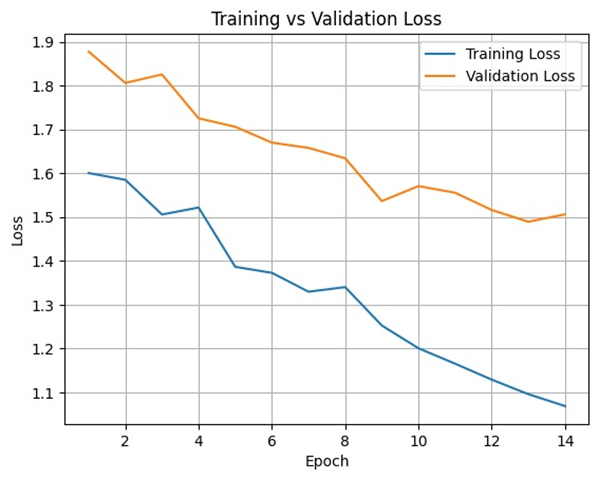
\includegraphics[width=0.5\linewidth]{train_val_loss.png}
    \caption{\textit{Average Training vs Validation Loss for 14 EPOCHS}
    \label{fig:avg-training-loss}
}
\end{figure}

The testing procedure for Florence-2 object detection model consists of a systematic multi-stage pipeline that evaluates model performance across various images. A testing pipeline consists of model prediction generation using Florence-2 followed by output processing to extract usable boxes and labels and ends with mAP evaluation besides confusion matrix display and per-class precision assessment. By implementing this evaluation process both benchmark assessment and visual verification of test images can be achieved through bounding box overlays on test images.The model testing process starts by creating empty lists for storing target annotations as targets1 while reserving prediction storage as predictions1. A progress bar controls the loop that  processes each test dataset sample through the tqdm library. The program retrieves the prefix prompt and suffix ground truth annotation from every image within the dataset. The input tensors needed by the model become possible through the processing abilities of the Florence-2 processor.  

After text prediction generation the model applies an LMM object detection structure from Florence-2 to translate these predictions into bounded boxes. The system selects predictions that display the specified classes while utilizing predefined category order to assign corresponding class IDs. To simplify evaluation processes the model administrator sets all predictions to have confidence scores of 1.0. The annotation decoding process for ground truth matches exactly the prediction decoding steps. The evaluation relies on the merged lists of targets and predictions for assessment. The system maintains continuous testing operation by printing descriptive error messages independently of overall evaluation termination when exceptions occur from either inference failures or malformed data.  

The implementation of plot\_bbox uses matplotlib and patches to offer visual support for numerical evaluation. The visualization function applies predicted bounding boxes and class labels to test images so they can be superimposed. The program generates red drawing boxes which display the class labels through semi-transparent backgrounds to make them visible. The visualization process executes sequentially through every prediction within the test set so manual verification can take place for each result. This stage gives developers and researchers the ability to examine model predictions visually to check accuracy and discover incorrect predictions then debug the model program. The visualization process detects all unexpected conditions and records them to prevent data or format inconsistencies from causing system crashes. 

\subsubsection{Real-Time Testing with Webcam Feed}

The research extends static evaluation by testing the model through real-time deployment of a live webcam video feed Fig.~\ref{fig:webcam}. The webcam stream comes into OpenCV which feeds each frame to the Florence-2 LoRA-enhanced model for prediction purposes. A text output parsing engine based on regular expressions retrieves object classes together with bounding box coordinates from model responses. The normalized coordinates output from Florence-2 are properly adjusted based on webcam frame dimensions that span from 0 to 999. The model annotates detected objects by assigning class names and overlaying boxes in randomly assigned colors to differentiate the objects. The application provides online display of annotated frames by allowing users to stop the loop with the Escape key. The system provides evidence for the model’s ability to apply its generalization capabilities to unrecognizable real-world situational frameworks for practical surveillance and robotics missions. 

\begin{figure}[H]
    \centering
    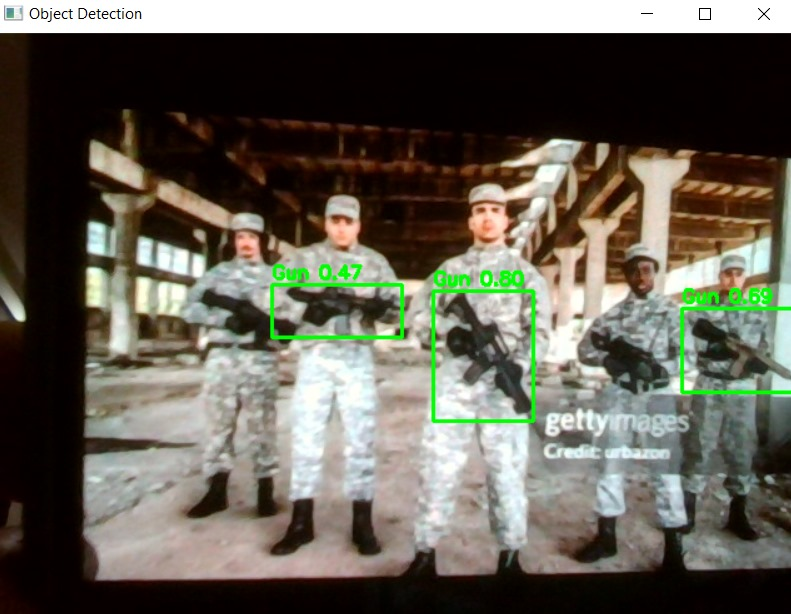
\includegraphics[width=0.5\linewidth]{webcam_result2.png}
    \caption{Real-time Detection on Webcam}
\end{figure}

\subsubsection{Quantization \& Pruning}

Model optimization methods specifically designed for deep learning comprise quantization and pruning which help deploy deep learning models onto edge devices using their limited processing resources. The strategies minimize model size alongside complexity while maintaining performance standards which qualify models for Raspberry Pi 5 restricted hardware platforms. Model weights from Florence-2 LoRA received optimizational adjustments through quantization and pruning methods to achieve reduced file size which started from around 1GB. The efficiency deployment happened while maintaining below-average performance losses.  

The decrease in precision levels of model parameters and activations constitutes quantization that transforms high-precision FP32 floating-point into lower-precision forms such as 16-bit FP16 or 8-bit integer INT8. Lower precision levels decrease memory requirements while decreasing the computational needs which results in improved inference speed performance. Hardware selection determines which quantization algorithms will be implemented according to expected performance levels. The method of weights quantization for real-time execution with FP32-kept activations stands as the preferred choice when using CPUs for prediction operations. Static quantization requires calibration data for accuracy compensation while it includes weight and activation quantization. During Quantization-aware training (QAT) the system uses simulated quantization effects during the training process which maximizes performance but requires increased training duration. The linear layers in Florence-2 LoRA implemented dynamic quantization which produced optimal performance-speed tradeoffs.  

The mathematical representation of INT8 quantization involves mapping each floating point value x to an 8-bit integer q using the equation:  

\textbf{Quantization:} The floating-point input $x$ is quantized to an integer representation $\hat{x}$ using a scale factor $s$ and zero-point $z$:

\begin{equation}
\hat{x} = \text{round}\left( \frac{x}{s} \right) + z
\end{equation}

where $s$ is the scale factor that maps floating-point values to integers, and $z$ is the zero point used to handle non-zero minimum values. This mapping ensures minimal accuracy loss while reducing memory footprint.

The optimization technique of pruning removes all unnecessary parameters that exist in the model framework. The model retains its essential performance without experiencing any losses when the unnecessary parameters are removed. The pruning process contains two types: unstructured pruning which removes individual weights to form sparse matrices and structured pruning which eliminates full neurons, filters or channels. Global pruning focuses on the least significant weights throughout the model. 
A pruning operation was conducted on Florence-2 LoRA linear layers where 50\% of weights were removed from each layer according to their L1 norm values. The selected weight elimination method protects model performance metrics while achieving significant compression of the size.

The L1 norm used to determine the importance of weights is calculated as:

\begin{equation}
\| w \|_1 = \sum_{i=1}^{n} |w_i|
\end{equation}


where $w_i$ represents individual weight values. Lower L1 norms indicate less influential weights, making them ideal candidates for pruning. By targeting these weights, the sparsity of the model is increased without affecting the more critical parameters.

The weights of the pruned model were quantified into small integer values (e.g., INT8) for deployment readiness and reduced memory requirements. These changes positioned the 5 model for real-time execution on Raspberry Pi 5. Both pruning and quantization produced a substantial improvement to the performance-scaled dimension relationship thus optimizing the solution which met edge computing requirements.

\begin{algorithm}
\caption{Dynamic Quantization of Florence-2 LoRA}
\label{alg:dynamic_quant}
\noindent\textbf{Input:} Checkpoint path $C$, model $M$
\begin{algorithmic}[1]
\State \textbf{// Load model $M$ from checkpoint path $C$}
\State $model \gets \text{torch.load}(C,\ \text{map\_location} = \text{"cpu"})$
\State \textbf{// Apply dynamic quantization to linear layers}
\State $quantized\_model \gets \text{quantize\_dynamic}( $
\hspace{2em}$model,$

\hspace{2em}$\{\text{torch.nn.Linear}\},$ \textbf{// Target linear layers}

\hspace{2em}$\text{dtype} = \text{torch.qint8}$ \textbf{// Use INT8 for compression}

$)$
\State \textbf{// Save the quantized model $M_q$}
\State $\text{torch.save}(quantized\_model.\text{state\_dict}(),\ \text{"florence2\_lora\_quantized.pt"})$
\end{algorithmic}
\noindent\textbf{Output:} Quantized model $M_q$
\end{algorithm}


Once trained the process extracts the model from its checkpoint as shown in Algorithm~\ref{alg:dynamic_quant}, before carrying out dynamic quantization on the linear layers for conversion into efficient 8-bit integers (INT8). After placement, the converted model receives storage for deployment as it functions well on resource-limited edge devices such as Raspberry Pi. 

\begin{algorithm}
\caption{L1 Unstructured Pruning of Quantized Model}
\label{alg:l1_pruning}
\noindent\textbf{Input:} Quantized checkpoint path $C_q$, model $M_q$
\begin{algorithmic}[1]
\State \textbf{// Load the quantized model $M_q$ from checkpoint path $C_q$}
\State $model \gets \text{torch.load}(C_q,\ \text{map\_location} = \text{"cpu"})$
\State \textbf{// For each module in model:}
\For{$name, module \in model.\text{items()}$}
    \State \textbf{// If the module is of type Linear:}
    \If{$\text{isinstance}(module,\ \text{torch.nn.Linear})$}
        \State \textbf{// Prune the weights of the module:}
        \State $\text{prune.l1\_unstructured}( $
        
        \hspace{2em}$\text{module},$ \textbf{// Target module}
        
        \hspace{2em}$\text{name} = \text{"weight"},$ \textbf{// Target weights}
        
        \hspace{2em}$\text{amount} = 0.5$ \textbf{// Prune 50\% of weights}
        
        $)$
    \EndIf
\EndFor
\State \textbf{// Save the pruned model $M_p$}
\State $\text{torch.save}(model,\ \text{"florence2\_lora\_quantized\_pruned.pt"})$
\end{algorithmic}
\noindent\textbf{Output:} Pruned model $M_p$
\end{algorithm}


The quantized model Algorithm~\ref{alg:l1_pruning} goes through an operation that applies L1 unstructured pruning to eliminate 50\% of its least important weights for further model compression. The performance remains unaffected by this method while it lowers both the computational requirements and storage needs. After reduction the lightweight model gets stored for future deployment. 

\subsection{Deploying Model on Raspberry Pi 5 Processor}

The Raspberry Pi 5 Fig.~\ref{fig:hardware-deployment} operates as the essential processor which functions as both a computing center and edge processing hub for delivering instant artificial intelligence-based threat alerts within minimally equipped distant areas. Its compact board design permits execution of advanced artificial intelligence models across low-power operation systems deployed in field areas thus creating a perfect solution for edge-based inference applications. The latest Raspberry Pi 5 model represents the top version of its series with upgraded features that increase computing outputs and system efficiency beyond prior models. The 64-bit quad-core Arm Cortex-A76 processor inside the device reaches operating speeds of 2.4 GHz which provides 2–3 times better performance than the Raspberry Pi 4. The processor achieves out-of-order execution capabilities in its architecture which enables effective handling of complex AI inference operations with enhanced responsiveness together with shortened latency.

A Raspberry Pi 5 provides ideal performance for this project because it offers a good combination of calculation power alongside compact dimensions and economical pricing and energy conservation. Within the system framework these are the main duties of the Raspberry Pi 5.

\begin{itemize}
    \item AI Model Hosting and Inference: Local execution of the optimized Florence v2 ViT-based vision model takes place through the Raspberry Pi 5. The deployed model runs on simple inference code bases including TensorFlow Lite and ONNX Runtime to detect drones together with handheld weapons and camouflaged items. Model quantization and pruning optimization methods reduce both memory requirements and inference durations allowing the model to operate effectively on device systems without impacting detection performance.
    \item Image Processing and Threat Detection: Real-time object classification and detection occur when the Pi 5 receives video frames from its connected camera module while processing the data before processing these inputs through the AI model. The system performs all processing directly on its hardware thus eliminating the need for cloud-based servers to enhance detection response speed.
    \item Integration with ESP32-S2 for Communication: Through the connection of Raspberry Pi 5 to the ESP32-S2 microcontroller it enables alert transmission with ESP-NOW protocol. The ESP-NOW protocol provides efficient peer-to-peer connectionless communication for low-power data transfer operations that work without requiring a standard Wi-Fi infrastructure. The Pi 5 transmits both detection alerts and inference results to the ESP32-S2 through GPIO or UART interface before it continues wireless transmission.
    \item Power Management and Portability: The Pi 5 includes features for operation with battery power which enables surveillance capabilities to continue throughout field-based deployments. The device operates using solar-powered systems and portable lithium-ion battery packs which support moving operations and remote functionality.
    \item Expandability and Customization: Through its 40 GPIO pins and HAT support the system enables developers to easily connect IR and PIR and ultrasonic sensors and buzzer and light actuators along with other IoT devices. The system allows users to adapt its functionality in multiple ways due to its flexible design for surveillance and monitoring needs.
\end{itemize}

\begin{figure} [H]
    \centering
    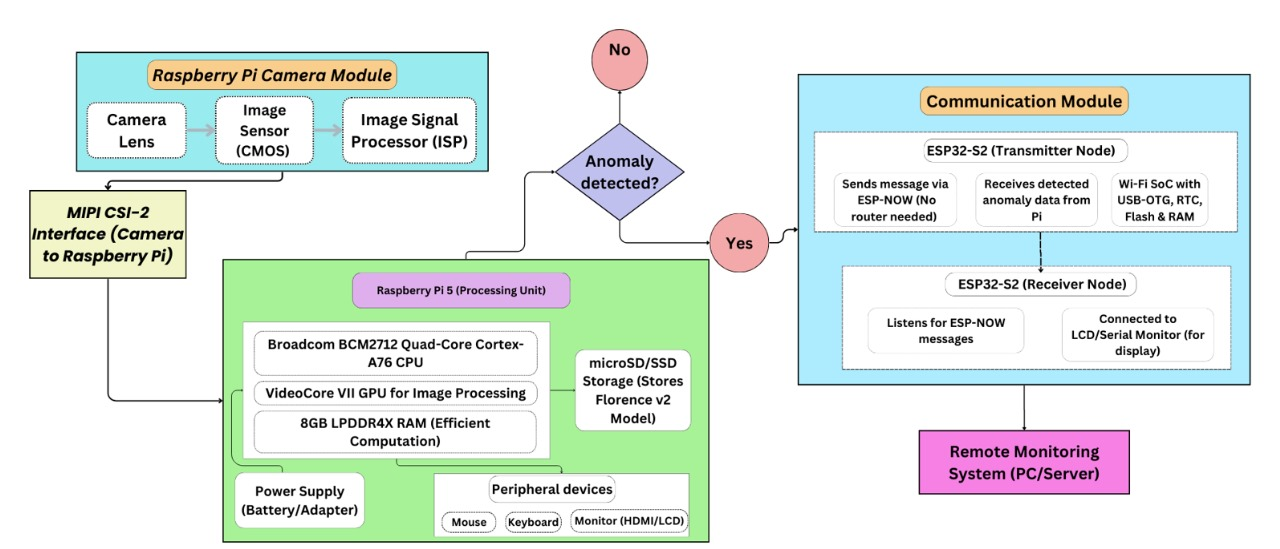
\includegraphics[width=1\linewidth]{hardware_architecture}
    \caption{Hardware Deployment Setup Featuring Raspberry Pi 5 and ESP32S2}
    \label{fig:hardware-deployment}
\end{figure}

The Raspberry Pi 5 serves as the core computing device that runs Florence v2 Vision Transformer for detecting military-grade threats. The system receives real-time high resolution images through the Raspberry Pi Camera Module attached to a connected Raspberry Pi. The system transmits the frames to the Florence v2 model for examination through its temporary buffer mechanism. Each frame in the Florence v2 system undergoes processing through its Vision Transformer architecture by splitting the input into defined sections called patches. The system distributes image information into patches which undergo successive self-attention procedures followed by feed forward operations. The model processes global image information which allows it to detect hidden threats including compact objects such as drones and handheld weapons.The pipeline analysis generates an output which tells if there is an anomaly present within the frame.

The main reason for using Raspberry Pi 5 stem from its compact design and efficient AI workload management at field level. Model performance optimization through pruning and quantization techniques makes the deployment possible for Raspberry Pi hardware systems maintaining accuracy levels. The deployed system performs continuous frame analysis and indicates real-time anomaly detections. The system recordings go through a process that sends alerts to the subsequent module. 

\subsection{Alert Transmission using ESP32S2 Module}
When an anomaly occurs the Raspberry Pi triggers a communication program that starts transmission to the ESP32-S2 module. The system employs this microcontroller to serve as an energy-efficient wireless transmitter which delivers live alerts independently from typical network systems. The ESP32-S2 module operates with ESP-NOW protocol as developed by Espressif which serves as the connectionless communication protocol for this configuration. The ESP-NOW protocol enables diverse devices to share information efficiently along with low-power performance that makes it suitable for remote area surveillance deployments. One unit of ESP32-S2 functions as the transmitting node connected to Raspberry Pi which communicates with another ESP32-S2 unit acting as a receiving node linked to the monitoring station PC.Programming for the ESP32-S2 transmitting module occurs through utilization of the Arduino IDE. The Raspberry Pi alerts the transmitter with either a GPIO signal or serial data format for anomaly data before the ESP-NOW wireless protocol goes into action.The signal acquisition and alert transmission from the second ESP32-S2 module leads to PC-based alert presentation which operators can view or record. The arrangement creates rapid power-efficient data transfer across extensive ranges of distances 
particularly in regions where Wi-Fi or cellular networks either lack availability or experience instability. 

ESP-NOW protocol provides additional reliability to systems by removing the 
requirement of authentication procedures while shortening response times when operating during critical emergencies. The Raspberry Pi 5 module teams up with the ESP32-S2 modules to create a self-sufficient edge-based surveillance system that remains price-effective and compact. Through their combined hardware capabilities this platform operates autonomously in live conditions to detect security threats before quickly sending out alerts which boosts defense forces plus civilian monitoring units readiness to handle situations.

\begin{figure}[H]
    \centering
    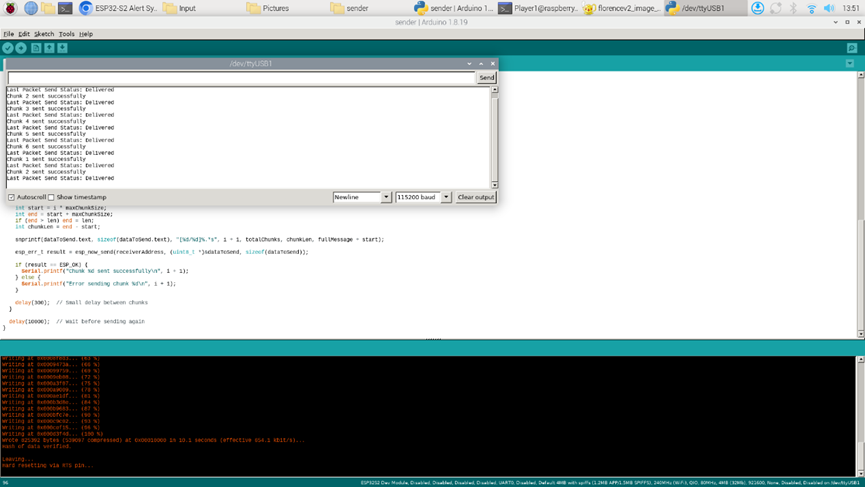
\includegraphics[width=1\linewidth]{esp32s2_1.png}
    \caption{Transmitting Alert through ESP32S2 module }
    \label{fig:transmitting-alert}
\end{figure}

The smart drone uses the onboard object detection module which transmits real-time annotated output images to the ESP32-S2 microcontroller. The images present detection results through boxes which indicate boundaries and names of recognized entities. The generated output visualization proceeds from the deep learning model inference phase before the transmission occurs through Wi-Fi for observation. The drone processing frames reveals its precise aerial target localization and classification abilities which validates both edge processing and lightweight transmission features Fig.~\ref{fig:transmitting-alert} of the ESP32-S2 microcontroller Fig.~\ref{fig:receiving-alert}. 

\begin{figure}[H]
    \centering
    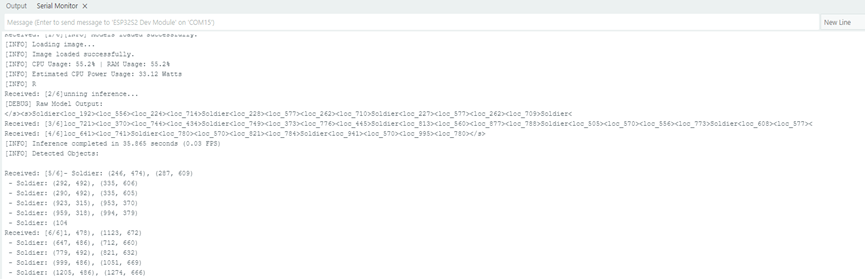
\includegraphics[width=1\linewidth]{transmit_2.png}
    \caption{Receiving Alert on Private PC}
    \label{fig:receiving-alert}
    
\end{figure}

\section{ANALYSIS OF STUDY AND RESULTS}

The research performed a detailed assessment of Florence v2 as a unified vision-language foundation model dedicated to aerial surveillance and object detection capabilities in Fig.~\ref{fig:obj-florence-detected} and Fig.~\ref{fig:results-detected}. The evaluation assessed how accurately the model detected targets while measuring its operational speed and visual signal recognition skills in complicated observation areas. Quantitative measurement outputs alongside visual assessments show that Florence v2 successfully performs drone image understanding and classification tasks for intelligent surveillance use.

\begin{figure}
    \centering
    \includegraphics[width=1\linewidth]{Output_collage.png}
    \caption{Results received from trained Florence Model}
    \label{fig:results-detected}
\end{figure}

\begin{figure} [H]
    \centering
    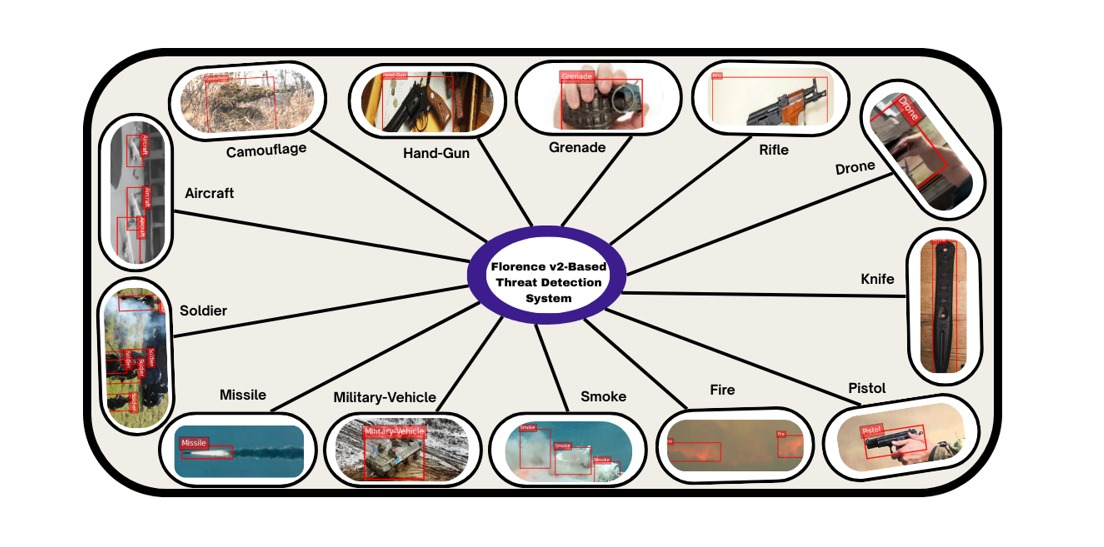
\includegraphics[width=1\linewidth]{detections.jpg}
    \caption{Objects Detected by FlorenceV2 with Bounding Box}
    \label{fig:obj-florence-detected}
\end{figure}

\subsection{FLORENCE V2 RESULTS ANALYSIS}

Table~\ref{tab:ddqn_metrics} shows Florence v2's class-wise accuracy performance on the military object detection dataset. Florence v2 performs better detection with 100\% accuracy in most of the major object classes like Aircraft, Drone, Grenade, Hand-Gun, Military-Vehicle, and Pistol. These accuracies reflect the model's capacity to detect well-defined and distinguishable objects. Other classes such as Knife (90.91\%), Camouflage (86.67\%), and Soldier (85.71\%) also perform well, indicating the robustness of the model even for scenes with partial occlusions or complex backgrounds. But classes such as Rifle (63.64\%), Smoke (68.42\%), and Fire (72.00\%) are less precise, possibly because of the visual ambiguity, low contrast, or fewer training images. 

\begin{table}[H]
\centering
\caption{Class-wise Accuracy of Florence v2 }
\renewcommand{\arraystretch}{1.5} % Row padding
\setlength{\tabcolsep}{12pt} % Column padding
\begin{tabular}{|c|c|}
\hline
\textbf{Class} & \textbf{Florence v2 Accuracy (\%)} \\
\hline
Aircraft           & 100.00 \\
Camouflage         & 86.67  \\
Drone              & 100.00 \\
Fire               & 72.00  \\
Grenade            & 100.00 \\
Hand-Gun           & 100.00 \\
Knife              & 90.91  \\
Military-Vehicle   & 100.00 \\
Missile            & 76.92  \\
Pistol             & 100.00 \\
Rifle              & 63.64  \\
Smoke              & 68.42  \\
Soldier            & 85.71  \\
\hline
\textbf{Average Accuracy} & \textbf{88.02} \\
\hline
\end{tabular}
\label{tab:ddqn_metrics}
\end{table}

In spite of these difficulties, Florence v2 has a highly accurate mean of 88.02\%, which is a very dependable option for real-time object detection in hazardous and dynamic situations like defense systems or military surveillance.

By combining observations from the accuracy trend in Fig.~\ref{fig:accuracy-50img} and the confusion matrix in Fig.~\ref{fig:confusion-matrix}, we can assert that the model indicates general strong classification performance in general, particularly after the first couple of samples. While cumulative accuracy levels off at a high and stable level, the confusion matrix indicates specific class-level problems, particularly with visually confused classes. Addressing these patterns of confusion through targeted model fine-tuning or preprocessing data might still enhance overall performance and reduce misclassifications.

\begin{figure} [H]
    \centering
    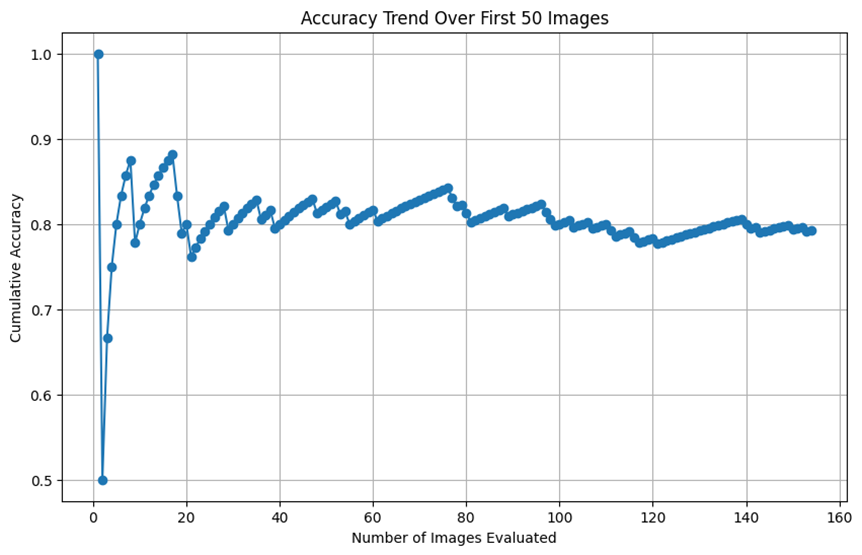
\includegraphics[width=1\linewidth]{accuracy.png}
    \caption{Accuracy Trend over first 50 images}
    \label{fig:accuracy-50img}
\end{figure}

Table~\ref{tab:florence_classification} illustrates a fine-grained classification report for Florence v2, indicating its performance on 13 object categories under the primary evaluation metrics: precision, recall, F1-score, and support. The model demonstrates perfect precision, recall, and F1-score (1.00) on classes like Aircraft and Hand-Gun, confirming Florence v2's capability to accurately and reliably recognize those objects without producing false positives or negatives. Other top scoring classes are Military-Vehicle (F1: 0.96), Drone (F1: 0.95), and Camouflage (F1: 0.93) and have excellent generalization even under adverse visual conditions.


\begin{table}[H]
\centering
\caption{Classification Report of Florence v2}
\renewcommand{\arraystretch}{1.2}
\begin{tabular}{|p{2cm}|p{2cm}|p{2cm}|p{2cm}|p{2cm}|}
\hline
\textbf{Class} & \textbf{Precision} & \textbf{Recall} & \textbf{F1-Score} & \textbf{Support} \\
\hline
Aircraft           & 1.00 & 1.00 & 1.00 & 13  \\
Camouflage         & 1.00 & 0.87 & 0.93 & 15  \\
Drone              & 1.00 & 0.90 & 0.95 & 10  \\
Fire               & 0.78 & 0.70 & 0.74 & 20  \\
Grenade            & 0.73 & 0.73 & 0.73 & 11  \\
Hand-Gun           & 1.00 & 1.00 & 1.00 & 10  \\
Knife              & 0.20 & 0.50 & 0.29 & 4   \\
Military-Vehicle   & 0.92 & 1.00 & 0.96 & 12  \\
Missile            & 1.00 & 0.77 & 0.87 & 13  \\
Pistol             & 0.40 & 0.67 & 0.50 & 6   \\
Rifle              & 1.00 & 0.64 & 0.78 & 11  \\
Smoke              & 0.79 & 0.65 & 0.71 & 23  \\
Soldier            & 0.45 & 0.83 & 0.59 & 6   \\
\hline
\textbf{Accuracy}      &       &       & \textbf{0.79} & \textbf{154} \\
\textbf{Macro Avg}     & 0.79  & 0.79  & 0.70          & 154 \\
\textbf{Weighted Avg}  & 0.85  & 0.79  & 0.75          & 154 \\
\hline
\end{tabular}
\label{tab:florence_classification}
\end{table}

But performance degradation is observed in classes such as Knife (F1: 0.29) and Pistol (F1: 0.50) due to fewer instances (support = 4 and 6 respectively) or visual resemblance to other small shapes, thereby resulting in more misclassifications. Soldier and Smoke classes also have lower F1 scores of 0.59 and 0.71, reflecting the difficulty in classifying partially occluded or irregularly shaped objects.
 
In summary, the model performs an acceptable accuracy of 79\% on 154 test samples. A macro average F1-score of 0.70 indicates well-balanced performance in all classes, while a weighted average F1-score of 0.75 highlights the superb performance of the model on classes with high support. These results confirm Florence v2's performance for multi-class object detection in rich, real-world military scenes, with some of the areas noted as possible improvement opportunities using data augmentation or class balancing.

\begin{figure} [H]
    \centering
    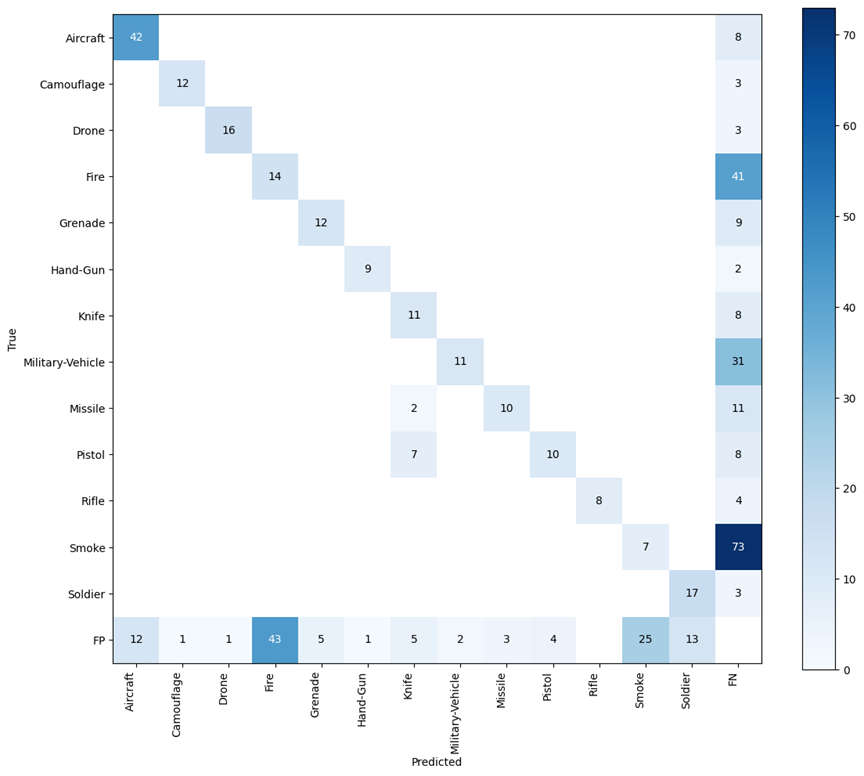
\includegraphics[width=1\linewidth]{confusion_matrix.png}
    \caption{Confusion Matrix of Florence v2 Predictions}
    \label{fig:confusion-matrix}
\end{figure}

The confusion matrix demonstrates a breakdown of the model's performance in classifying multiple classes like "Aircraft", "Fire", "Military-Vehicle", and "Soldier" in detail. The majority of classes, similar to "Aircraft" and "Drone", have high true positive values, indicating strong performance in classification. Some classes like "Fire" and "Soldier" have higher false positive and false negative values, indicating possible confusion with visually or contextually close categories like "Smoke" or "Military-Vehicle". Interestingly, "Smoke" and "Fire" are highly overlapping in misclassification, which is presumably because the two are visually similar and therefore may require further data augmentation or feature extraction refinement for those classes. The accuracy trend plot, "Accuracy Trend Over First 50 Images", indicates that the cumulative accuracy of the model fluctuates as it processes larger numbers of images. Accuracy is very unstable in the beginning, as it captures the high prediction performance variance on initial samples. But after the first 30 images, the accuracy becomes stable at around 80–85\%. This stability indicates that the model classifies well consistently after training on a small number of samples, showing a generally good classification ability with some initial instability.

\subsection{COMPARISON WITH STATE-OF-THE-ART MODELS}

Table~\ref{tab:compact_model_comparison} evidently indicates the better performance of Florence v2 over baseline object detectors such as YOLOv8, YOLOv12, Faster R-CNN, and Mask R-CNN.    Florence v2 boasts the best overall mAP50 of 70.92\%, which is considerably the highest, followed closely with great accuracy in difficult and high-priority classes such as Drone (92.77\%), Fire (99.50\%), Military-Vehicle (94.03\%), and Soldier (95.27\%). Even with the improvements of YOLOv12 over YOLOv8, that is, generalizing to more classes, it is still less than Florence v2 in terms of overall accuracy and reliability. The performance of Florence v2 demonstrates its efficiency and reliability for military object detection tasks, particularly in cases involving high recall and fine-grained class discrimination.

\begin{table}[H]
\centering
\scriptsize % Adjust font size to make everything smaller
\caption{Comparison of Class-wise Accuracy \& mAP50 across Detection Models}
\renewcommand{\arraystretch}{1.2} % Reduces row padding for compactness
\begin{tabular}{|p{1.2cm}|p{1cm}|p{0.7cm}|p{0.5cm}|p{0.5cm}|p{0.5cm}|p{0.5cm}|p{0.5cm}|p{0.5cm}|p{0.5cm}|p{0.5cm}|p{0.5cm}|p{0.5cm}|p{0.5cm}|p{0.5cm}|p{0.5cm}|}
\hline
\textbf{Method} & \textbf{Dataset} & \textbf{mAP} & \textbf{Air-craft\newline} & \textbf{Cam-ouf-lage\newline} & \textbf{Dro-ne\newline} & \textbf{Fire\newline} & \textbf{Gre-nade\newline} & \textbf{Han
d-Gun\newline} & \textbf{Kni-fe\newline} & \textbf{Mili
tary-\newline Veh
icle} & \textbf{Mis-sile\newline} & \textbf{Pis-tol\newline} & \textbf{Rif-le\newline} & \textbf{Smo-ke\newline} & \textbf{Sol-dier\newline} \\
\hline
Yolov8       & yolov8        & 45.5 & 44.9 & 58.2 & 61.5 & 6.1  & 82.3 & 72.7 & 65.3 & 59.8 & 17.4 & 87.7 & 75.7 & 4.9  & 50.7 \\
Yolov12      & yolov12       & 53.1 & 66.9 & 75.8 & 71.4 & 9.4  & 95.7 & 74.3 & 85.7 & 48.5 & 35.3 & 90.3 & 72.2 & 21.6 & 59.3 \\
F-RCNN       & COCO          & 45.0 & 17.9 & 30.1 & 18.3 & 3.2  & 57.6 & 28.4 & 41.4 & 43.6 & 1.6  & 27.9 & 43.6 & 0.8  & 25.1 \\
M-RCNN       & COCO          & 49.3 & 21.4 & 34.5 & 22.2 & 3.2  & 56.9 & 37.7 & 40.9 & 36.7 & 4.3  & 36.3 & 37.1 & 0.6  & 29.3 \\
Florence\newline V2 & Flor2-od & 70.9 & 65.4 & 92.8 & 99.5 & 25.4 & 82.0 & 88.6 & 94.0 & 36.2 & 39.3 & 90.6 & 92.9 & 19.9 & 95.3 \\
\hline
\end{tabular}
\label{tab:compact_model_comparison}
\end{table}

Table~\ref{tab:model_comparison} presents a comparative analysis of five object detection models—YOLOv8, YOLOv12, Faster R-CNN, Mask R-CNN, and Florence v2—compared in terms of critical performance and efficiency criteria. These are inference time per image, frames per second (FPS), training data format used, total and trainable parameters, and overall classification accuracy. Florence v2 shows ideal detection accuracy (88.02\%) vs computational expense, even though it has significantly more parameters. YOLOv12 has more accurate results (78.80\%) compared to YOLOv8 (70.89\%), though with the expense of slower inference time. Legacy models such as Faster R-CNN and Mask R-CNN have slower inference times and do not have a published accuracy here in this table, with the Florence v2 model being most accurate and the best choice among the models listed for real-time complex object detection tasks.

\begin{table}[H]
\centering
\caption{Performance \& Efficiency Comparison of Detection Models}
\small % or \normalsize
\renewcommand{\arraystretch}{1.15}
\setlength{\tabcolsep}{0.5pt}
\begin{tabular}{|c|c|c|c|c|c|c|}
\hline
\textbf{Model} & \textbf{Inference\newline Time (s)} & \textbf{Inference\newline Speed (FPS)} & \textbf{Dataset\newline Format} & \textbf{Total\newline Parameters} & \textbf{Trainable\newline Parameters} & \textbf{Accuracy\newline (\%)} \\

\hline
YOLOv8       & 0.0752 & 13.30 & yolov8         & \num{3157200}     & \num{3008183}     & 70.89 \\
YOLOv12      & 0.8557 & 1.17  & yolov12        & \num{2553904}     & -                & 78.80 \\
Faster-RCNN  & 0.2725 & -     & COCO           & \num{104441105}   & \num{104015953}  & -     \\
Mask-RCNN    & 0.2777 & -     & COCO           & \num{104441105}   & \num{104015953}  & -     \\
FlorenceV2   & 0.2582 & 3.87  & florence2-od   & \num{272733896}   & \num{1929928}    & 88.02 \\
\hline
\end{tabular}
\label{tab:model_comparison}
\end{table}

This table lists the performance of some object detection models—YOLOv8, YOLOv12, Faster R-CNN, Mask R-CNN, and Florence v2—on test and validation datasets according to typical COCO evaluation metrics: mAP@50, mAP@75, and mAP@[50:95]. Vision Transformer-based Florence v2 posts the best marks in all except one metric, indicating higher localization accuracy and robustness, particularly with a validation mAP@50 of 70.92\% and a test mAP@50 of 67.10\%. YOLOv12 is continually improving over YOLOv8 on all the metrics, with improved generalization. 

However, other classical models such as Faster R-CNN and Mask R-CNN are worse on both the datasets, especially on tighter metrics such as mAP@[50:95], where Florence v2 performs much better than them. The obtained results support the effectiveness of the transformer-based detectors such as Florence v2 in performing high detection accuracy on difficult object detection tasks.

\begin{table}[H]
\centering
\caption{Evaluation of Detection Performance on Validation and Test Datasets}
\small
\renewcommand{\arraystretch}{1.2}
\setlength{\tabcolsep}{4pt}
\resizebox{\textwidth}{!}{%
\begin{tabular}{|c|c|ccc|ccc|}
\hline
\textbf{Method} & \textbf{Model} & \multicolumn{3}{c|}{\textbf{Validation Dataset}} & \multicolumn{3}{c|}{\textbf{Test Dataset}} \\
\cline{3-8}
& & \textbf{mAP@50} & \textbf{mAP@75} & \textbf{mAP@50:95} & \textbf{mAP@50} & \textbf{mAP@75} & \textbf{mAP@50:95} \\
\hline
YOLO & YOLOv8      & 45.462 & -      & 27.235 & 76.579 & 56.000  & 52.860 \\
YOLO & YOLOv12     & 53.119 & 35.205 & 34.526 & 78.666 & 66.625  & 60.845 \\
Faster RCNN & Detectron2 & 44.960 & 25.365 & 26.639 & 30.615 & 19.778  & 14.785 \\
Mask RCNN   & Detectron2 & 49.286 & 26.059 & 28.451 & 29.523 & 20.253  & 16.953 \\
ViTs & FlorenceV2  & 70.922 & 56.447 & 55.211 & 67.105 & 52.324  & 50.261 \\
\hline
\end{tabular}%
}
\label{tab:map_comparison}
\end{table}

Cross-table comparison of Tables~\ref{tab:compact_model_comparison}, ~\ref{tab:model_comparison}, and ~\ref{tab:map_comparison} reveals Florence v2's overall dominance over other conventional object detection models. The best class-wise mAP50 in all categories except one proves Florence v2's ability to handle a very large number of object classes with higher precision. Table~\ref{tab:model_comparison} emphasizes its strength in having high accuracy (88.02\%) and good inference speed (3.87 FPS) in Fig.~\ref{fig:inference}, despite having a large parameter size—exemplifying the effect of light fine-tuning methods such as LoRA.

\begin{figure} [H]
    \centering
    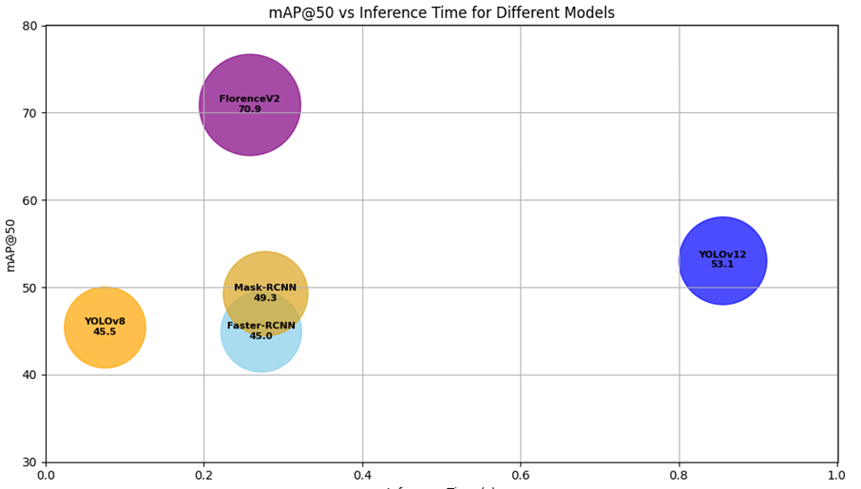
\includegraphics[width=1\linewidth]{compare.png}
    \caption{Inference Time vs. mAP of the Models in Military Object Detection}
    \label{fig:inference}
\end{figure}

Table~\ref{tab:map_comparison} further solidifies its dominance with leading mAP ranks on both the validation and test sets, which signify improved generalization performance. Together, these findings place Florence v2 as a stable and scalable object detection model for practical use.
The mAP@50 vs. inference time analysis graph in Fig ~\ref{fig:inference}. shows how the various models and their accuracy relates inversely to computational speed. The FlorenceV2 model holds both top performance and average inference speed reaching an mAP@50 rate of 70.92 while maintaining an inference time of 0.2582 seconds which suggests this model suits applications that require precise detection and quick response. YOLOv8 provides the fastest inference time at 0.0752 seconds yet has an mAP@50 value of 45.462 which makes it most suitable for applications needing real-time operation. YOLOv12 surpasses YOLOv8 in accuracy with an mAP@50 score of 53.119 but consumes approximately 0.8557 seconds of inference time thus showing a detection quality-focused trade-off. From among the region-based models Mask-RCNN demonstrates superior accuracy-speed performance by reaching an mAP@50 score of 49.286 with execution speed of 0.2777 seconds compared to Faster-RCNN which attains mAP@50 of 44.960 but remains equally slow. This demonstrates that YOLOv8 and Mask-RCNN deliver optimal speed for specific deployment needs but FlorenceV2 emerges as the best choice when maintaining high accuracy standards remains priority number one.

\subsection{HARDWARE PERFORMANCE ANALYSIS}

We have also tested Florence v2 on Raspberry Pi 5 with military image classification and results revealed strong performance limitations of edge devices. The model processed with 13 classes which include weapons such as rifles and grenades as well as environmental markers such as smoke and fire utilizing 16.6 seconds per inference step and a rate of 0.063 FPS. The system was seamless owing to minimal RAM usage at 38.4\% which was concurrent with stable CPU usage at 50.9\%. The test confirms that edge devices can execute vision models similar to Florence v2 to perform real-time threat alerts in operational activity.

\begin{table}[H]
\centering
%\footnotesize % Adjust font size to make everything slightly larger
\renewcommand{\arraystretch}{1.5} % Increases row padding for better spacing
\caption{Hardware Results with Florence v2 on Raspberry Pi}
\begin{tabular}{|p{2.5cm}|p{2cm}|p{2cm}|p{2cm}|p{2cm}|}
\hline
\textbf{Class} & \textbf{Inference Time (in seconds)} & \textbf{Average FPS} & \textbf{RAM Usage} & \textbf{CPU Usage} \\
\hline
Aircraft        & 15.436 & 0.065 & 31.9\% & 53.9\% \\
Camouflage      & 17.526 & 0.062 & 36.5\% & 54.7\% \\
Drone           & 15.681 & 0.060 & 39.2\% & 52.9\% \\
Fire            & 14.836 & 0.070 & 41.0\% & 57.4\% \\
Grenade         & 16.063 & 0.063 & 40.1\% & 52.6\% \\
Hand-Gun        & 18.115 & 0.060 & 38.6\% & 53.0\% \\
Knife           & 18.095 & 0.062 & 39.1\% & 53.2\% \\
Military-Vehicle & 16.640 & 0.060 & 38.9\% & 54.5\% \\
Missile         & 15.595 & 0.060 & 39.2\% & 55.1\% \\
Pistol          & 17.627 & 0.060 & 39.5\% & 52.8\% \\
Rifle           & 16.341 & 0.070 & 36.2\% & 52.7\% \\
Smoke           & 18.097 & 0.070 & 36.5\% & 15.3\% \\
Soldier         & 16.086 & 0.061 & 42.1\% & 53.2\% \\
\hline
Average         & 16.626 & 0.063 & 38.4\%  & 50.9\% \\
\hline
\end{tabular}
\label{tab:hardware_results}
\end{table}

All the available data in Table~\ref{tab:hardware_results} show that no previous research incorporates broad-range military class analysis and proven capabilities on low-hardware like the Raspberry Pi 5 device. Previous research either examines short subsets of classes and conducts their tasks on high-performance computing systems. The research achieves uniqueness by proving its model's readiness for actual edge deployment by experimenting with the Raspberry Pi 5 device for processing 13 important military objects.

\section{Conclusion}
This paper aims to showcase both the strengths and weaknesses of operating Transformer object detection models at the edge level. The deployment of Florencev2 supplied essential benefits that improved both interpretability capabilities and initial training accuracy levels. The system experienced deployment difficulties because of ONNX conversion imprecision combined with synthetic data restriction, hardware incompatibility, and poor communication infrastructure. 

The project achieved multiple essential targets despite facing different difficulties. A detection pipeline operating with a modified transformer model successfully executed object recognition tasks for predefined military object classes. ESP32-S2 wireless capability was tested and established in the project which created foundational knowledge for additional research about intelligent surveillance deployment methods. Technical challenges in this field require tighter connections between software frameworks and hardware systems because edge AI requires real-time image processing operational environments. 

This study provides valuable technical knowledge which points toward three key requirements that future edge AI deployment systems must address: model interoperability standards and light-weighted transformer engineering and secure deployment processes. The research and development community can benefit from the insights derived from this project because they strive to improve intelligent field surveillance systems.  


\section{Future Work}
Future work on various avenues presents the potential to strengthen the present system by improving scope and efficiency while increasing reliability levels. Future development needs to study better processes for ONNX export. The Florencev2 model delivers advanced performance capabilities yet building specialized converters and framework interfaces would help maintain high accuracy when deploying it on ONNX-friendly platforms. Working closely with developers who create model conversion platforms within open-source communities will speed up this development path. Data augmentation methods need to be enhanced in upcoming releases of the system for substantial benefit toward system advancement. Hybrid augmentation strategies combining diffusion models with style transfer methods or domain adaptation techniques should replace GANs for creating realistic training data especially when dealing with visually ambiguous categories like Camouflage. The system requires more real-world annotated images which can be obtained by domain-specific simulations or crowd-sourced labeling to solve present weaknesses and improve model robustness. 

Should be a main priority for future versions of the system to closely focus on hardware compatibility. The integration of camera modules with AI inference libraries would benefit from utilizing NVIDIA Jetson Nano or Coral Dev Board as well as low-power FPGA-based hardware systems. The modification would create improved real-time functions alongside better software-driver compatibility for smooth performance. The integration of wireless communication through LoRa requires future work to reattempt with updated modules or pre-certified LoRaWAN kits giving reliable firmware. The capability of achieving long-range low-power communication would become viable for rural defense control through this update. A resilience improvement for the system can be achieved through deploying a backup system that automatically changes between Wi-Fi (ESP32) mode and LoRa mode based on signal quality and battery health measurements.The future of surveillance development lays in combining different methods of sensor information. Other sensor systems including infrared and motion sensor systems and audio feed programs together with video data analysis would help create sustainable monitoring capabilities. Employing Florencev2 multi-modal embedding capability enables revolutionary opportunities that benefit threat classification apart from anomaly detection and environmental monitoring applications. 

A real-time display platform that presents operational status data together with system performance indicators and detection results and communication messages would be immensely useful for those working with and developing the system. The dashboard can function from either a local server setup or a secure cloud platform where users obtain monitoring and configuration control across a distance.

\printbibliography


\end{document}
